\section{Diseño de los programas}
\subsection{Red neuronal}
Por un lado, se utilizó el \href{https://docs.edgeimpulse.com/docs/tutorials/end-to-end-tutorials/responding-to-your-voice}{tutorial} de Edge Impulse para crear y entrenar una red neuronal que detecte los comandos por voz. Los comandos son \tt{lumos}, \tt{musica} y \tt{tele}. Además, se siguió los pasos del mismo tutorial para flashear el modelo en el Arduino Nano BLE 33 Sense. Esto quiere decir que el código necesario para crear, entrenar y flashear al Arduino el modelo fue generado automáticamente por Edge Impulse, por lo que todos los créditos van hacia Edge Impulse \cite{tutorial}, los autores de este reporte de laboratorio solamente hicieron uso de los scripts generado por Edge Impulse.

\begin{figure}
    \centering
    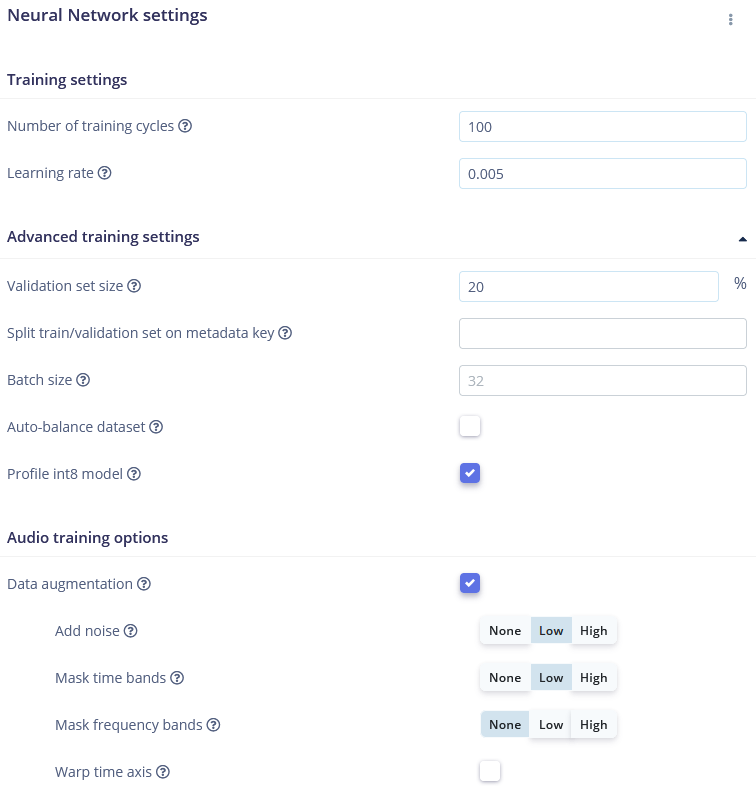
\includegraphics[width=12cm]{Imagenes/neural-1.png}
    \caption{Captura de pantalla de los parámetros de la red neuronal.}
    \label{neural-1}
\end{figure}

Además, los parámetros del modelo son las que Edge Impulse trae por defecto (figura \ref{neural-1}) así como recomendaciones que el tutorial menciona, cuya arquitectura de la red neuronal es el preset \tt{2D convolutional} (figura \ref{neural-2}) \cite{tutorial}. El código que se encarga de crear y entrenar la red se encuentra en el repositorio en la carpeta \tt{src/edge-impulse/} y el software necesario para flashear el modelo generado en el Arduino se encuentra en la carpeta \tt{src/firmware-arduino-nano-33-ble-sense/}.

\begin{figure}
    \centering
    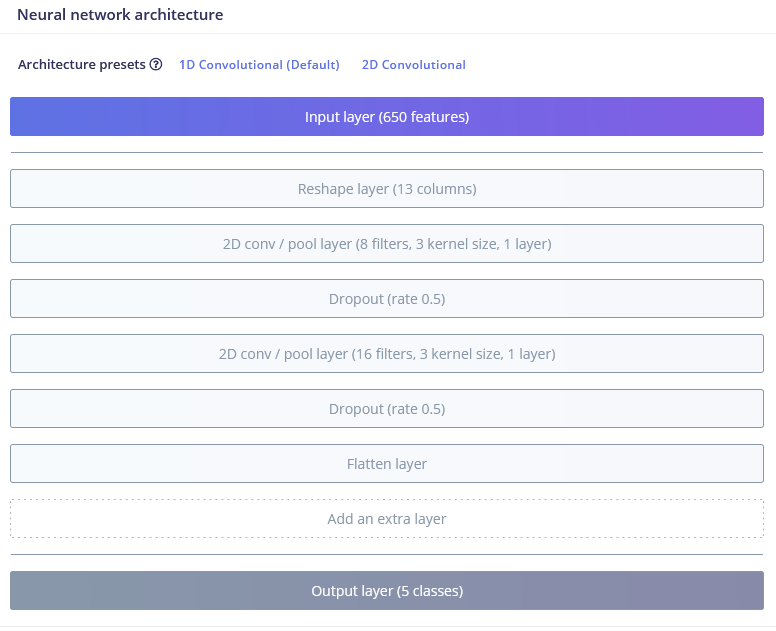
\includegraphics[width=12cm]{Imagenes/neural-2.png}
    \caption{Captura de pantalla de la arquitectura de la red neuronal.}
    \label{neural-2}
\end{figure}

\subsection{Diagrama de flujo del script de Python}
Por otro lado, se creó un script de Python (\tt{datos.py}) para poder recibir los datos del Arduino a la computadora. El diagrama de flujo se muestra en la figura \ref{py-diag}. La idea de este script es aprovechar que Edge Impulse tiene una interfaz en la terminal, esto es, tiene comandos para comunicarse con el Arduino. Tiene un comando denominado \tt{edge-impulse-run-impulse} que arroja en terminal las palabras, cuya cada palabra viene asociada un valor entre cero y uno. La palabra con el valor más alto es la palabra que el modelo cree lo que dijo el usuario \cite{edge-cli}.

\begin{figure}[th]
    \centering
    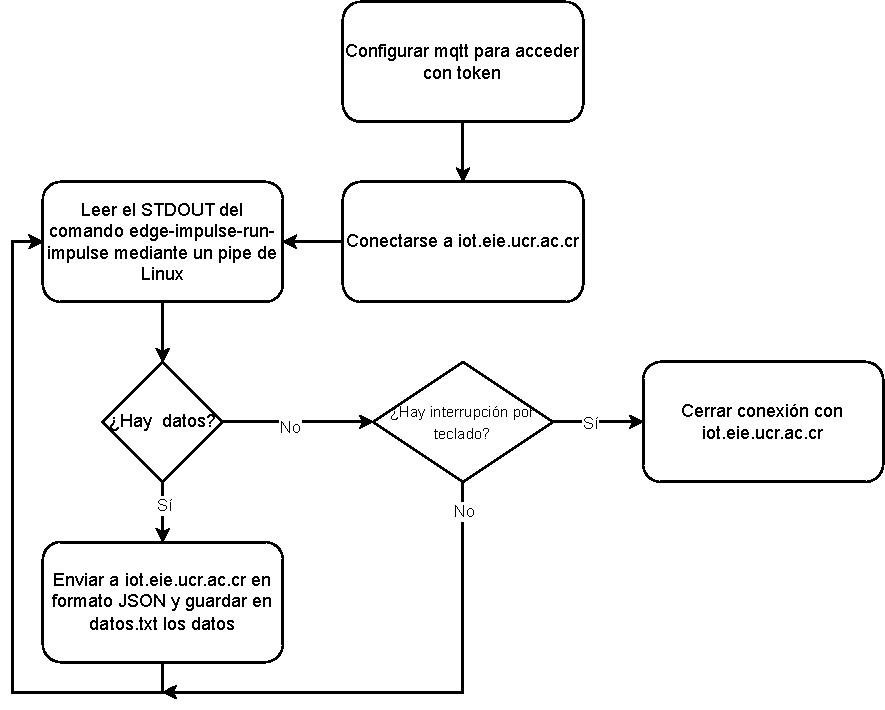
\includegraphics[width=13cm]{Imagenes/py.pdf}
    \caption{Diagrama de flujo del script para comunicar el Arduino con Thingsboard.}
    \label{py-diag}
\end{figure}

Ahora, mediante el pipe (\textbar) de Linux \cite{pipe} se puede redireccionar la salida del comando \tt{edge-impulse-run-impulse} a un script de Python en vez de arrojarlo en la terminal. Por lo tanto, lo que tendría que hacer el script de Python es recibir lo que \tt{edge-impulse-run-impulse} arroje y enviar a Thingsboard en formato JSON así como guardar en un archivo de texto las palabras con sus valores asociados. Por lo tanto, se debe correr \tt{edge-impulse-run-impulse --continuous | python3 datos.py} para poder recibir los datos del Arduino y guardalo en un archivo de texto así como enviarlo a Thingsboard. Sin embargo, el comando es largo y tedioso, así que el repositorio proporciona el script \tt{correr.sh} que ejecuta justamente ese comando para facilitar al usuario.